\documentclass[]{rptuseminar}

% Specify that the source file has UTF8 encoding
\usepackage[utf8]{inputenc}
% Set up the document font; font encoding (here T1) has to fit the used font.
\usepackage[T1]{fontenc}
\usepackage{lmodern}

% Load language spec
\usepackage[american]{babel}
% German article --> ngerman (n for »neue deutsche Rechtschreibung«)
% British English --> english

% Ffor bibliography and \cite
\usepackage{cite}

% AMS extensions for math typesetting
\usepackage[intlimits]{mathtools}
\usepackage{amssymb}
% ... there are many more ...


% Load \todo command for notes
\usepackage{todonotes}
% Sebastian's favorite command for large inline todonotes
% Caveat: does not work well with \listoftodos
\newcommand\todoin[2][]{\todo[inline, caption={2do}, #1]{
		\begin{minipage}{\linewidth-1em}\noindent\relax#2\end{minipage}}}

% Load \includegraphics command for including pictures (pdf or png highly recommended)
\usepackage{graphicx}

% Typeset source/pseudo code
\usepackage{listings}

% Load TikZ library for creating graphics
% Using the PGF/TikZ manual and/or tex.stackexchange.com is highly adviced.
\usepackage{tikz}
% Load tikz libraries needed below (see the manual for a full list)
\usetikzlibrary{automata,positioning}

% Load \url command for easier hyperlinks without special link text
\usepackage{url}

% Load support for links in pdfs
\usepackage{hyperref}

% Defines default styling for code listings
\definecolor{gray_ulisses}{gray}{0.55}
\definecolor{green_ulises}{rgb}{0.2,0.75,0}
\lstset{%
  columns=flexible,
  keepspaces=true,
  tabsize=3,
  basicstyle={\fontfamily{tx}\ttfamily\small},
  stringstyle=\color{green_ulises},
  commentstyle=\color{gray_ulisses},
  identifierstyle=\slshape{},
  keywordstyle=\bfseries,
  numberstyle=\small\color{gray_ulisses},
  numberblanklines=false,
  inputencoding={utf8},
  belowskip=-1mm,
  escapeinside={//*}{\^^M} % Allow to set labels and the like in comments
}

% Defines a custom environment for indented shell commands
\newenvironment{displayshellcommand}{%
	\begin{quote}%
	\ttfamily%
}{%
	\end{quote}%
}

%%%%%%%%%%%%%%%%%%%%%%%%%%%%%%%%%%%%%%%%%%%%%%%%%%%%%%%%%%%%%%%%%%%%%%%%%%%%%%%

\title{Seminar Template for Computer Science}
\event{Seminar: XXX in Summer term 2019}
\author{ Mohammadmehrdad Shahidi, Zahra Khodabakhshian 
  \institute{Technische Universität Kaiserslautern, Department of Computer Science}}

%%%%%%%%%%%%%%%%%%%%%%%%%%%%%%%%%%%%%%%%%%%%%%%%%%%%%%%%%%%%%%%%%%%%%%%%%%%%%%%
\begin{document}
%%%%%%%%%%%%%%%%%%%%%%%%%%%%%%%%%%%%%%%%%%%%%%%%%%%%%%%%%%%%%%%%%%%%%%%%%%%%%%%

\maketitle

%%%%%%%%%%%%%%%%%%%%%%%%%%%%%%%%%%%%%%%%%%%%%%%%%%%%%%%%%%%%%%%%%%%%%%%%%%%%%%%

\begin{abstract}
    Give an abstract of your paper. You may also give a very short explanation why it could be useful for the reader, i.~e.~ a short motivation.
\end{abstract}

%%%%%%%%%%%%%%%%%%%%%%%%%%%%%%%%%%%%%%%%%%%%%%%%%%%%%%%%%%%%%%%%%%%%%%%%%%%%%%

\section{Introduction}
\label{sec:introduction}

The introduction includes the motivation for the presented work.
In general, the author will explain the addressed problem and why it is of interest to solve that problem.
The most important thing is to explain the papers contribution, e.~g.~ a paper may introduce a new (more efficient) algorithm or/and the proof of an (existing) algorithm or just a method to solve the addressed problem.
A general introduction can not be given due to the diversity and variety of problems and their solutions.
Finally, the section can be closed by giving an overview of the rest of the paper.
E.~g.~ ``The rest of the paper is structured as follows:
Section \ref{sec:relatedwork} gives an overview of related work and existing solutions of the addressed problem. $\ldots$''

\section{Related Work}
\label{sec:relatedwork}

Related work is a very important part of a paper.
Basically, the reader has to be convinced that the author of a paper prepared himself carefully.
Existing work has to be cited and the author has to explain advantages/disadvantages and limitations of work that is similar to the presented work.
In particular, research is the keyword: the author is advised to use libraries or the internet to search for existing solutions of the addressed problem.
You are advised to connect sections by short sentences, e.~g.~ ``The next section introduces the solution of the addressed problem''.

\section{The Solution}
\label{sec:solution}

Whatever the addressed problem is: now the author can start to explain her/his work.
After the explanation, experiences, results or just a discussion of the presented work has to be given in Section \ref{sec:conclusions}.

\section{Conclusions, Results, Discussion}
\label{sec:conclusions}

This section will usually be the last section in a paper.
Authors may split results and conclusions into two separate sections.



\newpage

\section{How to install \LaTeX{}}

\begin{description}
 \item[Linux]
Your distribution will most likely offer a Latex package.
For Ubuntu you can install the \lstinline!texlive-full! package via:

\begin{displayshellcommand}
  sudo apt install texlive-full
\end{displayshellcommand}

\item[Mac]
Download and install the MacTeX distribution (\url{https://www.tug.org/mactex/}).

\item[Windows]
You can install TeX Live (\url{https://www.tug.org/texlive/windows.html}) or MiKTeX (\url{https://miktex.org/howto/install-miktex}).
\end{description}

Make sure that the \lstinline!latexmk! tool is also installed.
You can find installation instructions for \lstinline!latexmk! at \url{http://mg.readthedocs.io/latexmk.html#installation}.

There are also online editors with dedicated Latex support.
The SCI offers a free hosting of ShareLatex, the open-source equivalent to the commercial overleaf version.
Please check their webpage for more information.

\section{How to build this document}
In essence, building a \LaTeX{} document is as simple as running
\begin{displayshellcommand}
	latexmk -pdf seminar.tex
\end{displayshellcommand}
Here \lstinline!seminar.tex! is the name of the main \texttt{tex}-file.

The \lstinline!latexmk! tool integrates several tools including \lstinline!pdflatex! and \lstinline!biber!.
It makes sure that the individual tools are run in the right order and often enough.
If you (or your editor) run the individual tools remember that it might be necessary to compile multiple times.
For example, without \lstinline!latexmk! this document requires the following sequence of commands in order to get all citations and references right:
\begin{displayshellcommand}
  pdflatex seminar \\
  bibtex    seminar \\
  pdflatex seminar \\
  pdflatex seminar
\end{displayshellcommand}
Note that as long as no citations of bibliography data change between builds (and you do not delete any of the generated files) two runs of \texttt{pdflatex} are enough to rebuild the document.

\paragraph{Makefike} This template also contains a \lstinline!makefile!, so that this document can be compiled by running \lstinline!make!.
Moreover \lstinline!make watch! can be used to recompile the document whenever it changes.
The Makefile is also configured with Synctex, which enables some PDF-viewers to jump from the document to the correct position in the \LaTeX{} code.

\subsection{Editors}
\label{sec:editors}

There are a number of IDE-like \LaTeX{} editors (none of which fully satisfies the authors).
Most are basically a text editor with some gimmicks, but those can already facilitate writing \LaTeX{} documents significantly.
\begin{description}
	\item[TeXStudio] standalone editor with built-in pdf viewer
	(with source $\leftrightarrow$ pdf sync), automatic build, instant preview \dots
	\item[Kile] KDE-user's default choice
	\item[TeXlipse] Eclipse plugin for \LaTeX{} which is reasonably powerful.
	\item[Emacs with AUCTeX] If you like Emacs, this is what you want to use.
	\item[TeXShop] for MAC users
	\item[Your favorite text editor] probably has \LaTeX{} syntax highlighting at least.
	  Look for plugins that add more features.
\end{description}

\section{More on \LaTeX}
A whole collection of tutorials and further information is collected by the German \TeX{} user group~\cite{danteintro}.

We consider the following material especially useful:
\begin{itemize}
	\item \href{http://mirrors.concertpass.com/tex-archive/info/lshort/english/lshort.pdf}{``The Not So Short Introduction to \LaTeXe''}, a basic tutorial for \LaTeX{}.
	\item The \LaTeX{} cheat sheet at \url{http://www.stdout.org/~winston/latex/}.
	\item Overviews on typesetting mathematics are available on
	  \begin{itemize}
	    \item Wikibooks (\href{http://en.wikibooks.org/wiki/LaTeX/Mathematics}{en.wikibooks.org/wiki/LaTeX/Mathematics}),
	    \item Wikipedia (\href{http://en.wikipedia.org/wiki/Help:Displaying_a_formula}{en.wikipedia.org/wiki/Help:Displaying\_a\_formula}) and
	    \item Mathematics Stack Exchange (\href{http://meta.math.stackexchange.com/q/5020/3330}{meta.math.stackexchange.com/q/5020}).
	  \end{itemize}
	\item Access package documentation by executing \texttt{texdoc packagename} on shell (needs
	\href{https://www.tug.org/texlive/}{TeX Live}).
	\item Find symbols by drawing them with \href{http://detexify.kirelabs.org}{Detexify}.
	\item Command-line program \texttt{lacheck} is often better at detecting syntactical errors than the standard \texttt{pdflatex}
	itself; in fact \texttt{pdflatex}'s error messages are hardly ever useful.
	\item A very comprehensive and up-to-date repository of \LaTeX{} packages is
	  available on \href{http://ctan.org/}{CTAN}.
	\item If you want to use other fonts, visit the \href{http://www.tug.dk/FontCatalogue/}{\LaTeX{} Font Catalogue}. However, fonts can be a ficklish issue in \LaTeX{}, see also
	  \href{http://tex.stackexchange.com/q/25249/3213}{tex.stackexchange.com/q/25249}.
	\item For any \LaTeX{} question, visit \href{http://tex.stackexchange.com}{tex.stackexchange.com}.
\end{itemize}
Note that since \TeX{} and \LaTeX{} are decades old and many features have been added by packages over the years, lots of information on the internet are obsolete by now.
A famous example are umlauts and other ``non-standard'' character  (äöüßåø) which used to require special commands; nowadays these work out of the box with Unicode source files.
See the source of this document to see how it is done.

In case of doubt, we recommend visiting \href{http://tex.stackexchange.com}{TeX~--~LaTeX Stack~Exchange}; not only does the site cover many problems already but the community is very knowledgeable in all things \LaTeX{}.

\begin{figure}
\begin{lstlisting}[language=Scala,numbers=left]
def sort[T](list: List[T])(implicit ord: Ordering[T]): List[T] = {
  list match {
    case Nil => Nil
    case x :: xs =>
      // partition list based on pivot element x
      val (lo, hi) = xs.partition(ord.lt(_, x))  //*\label{srcline:algcmp}
      sort(lo) ++ (x :: sort(hi))
  }
}
\end{lstlisting}
\caption{An example algorithm. Do you recognize it? Line~\ref{srcline:algcmp} is crucial!}
\label{alg:example}
\end{figure}

There are also some particular features we consider noteworthy.
\begin{itemize}
  \item Referencing (things which have a \texttt{label}) and citing\footnote{Citations are defined in \lstinline!references.bib! as BibTeX entries.
    You can find BibTex entries on most web-pages where you can access papers and articles.}.
  For instance,
    \begin{itemize}
      \item ``\verb|See Section~\ref{sec:editors}|''
            compiles to ``See Section~\ref{sec:editors}'' and
      \item ``\verb|a tutorial~\cite{danteintro}|'' compiles to
            ``a tutorial~\cite{danteintro}''.
    \end{itemize}
    There are more commands (and packages) for finer control, such as \verb|\eqref|,
    \verb|\pageref|, \verb|\nameref| and \verb|\textcite|.

    The most convincing reason to use these is probably that~-- since links
    are computed given the current source~-- numbering, names and links survive
    rearrangements of the material.

  \item (Pseudo-)Code can be typeset by a number of packages, e.\,g.\ \texttt{listings}.
    See Listing~\ref{alg:example} for an example.
    % Note: see the preamble for some global configuration of listings

  \item With the \texttt{todonotes} package it is easy to leave little reminders in your document\todo{Should we explain more?}.
  \item TikZ is a great package for creating all sorts of graphics, see e.\,g.\ Figure~\ref{fig:tikz}.
    Find an extensive list of examples (with sources) on
    \href{http://www.texample.net/tikz/examples/}{texample.net/tikz/examples}.
    \begin{figure}
	    \begin{center}
		    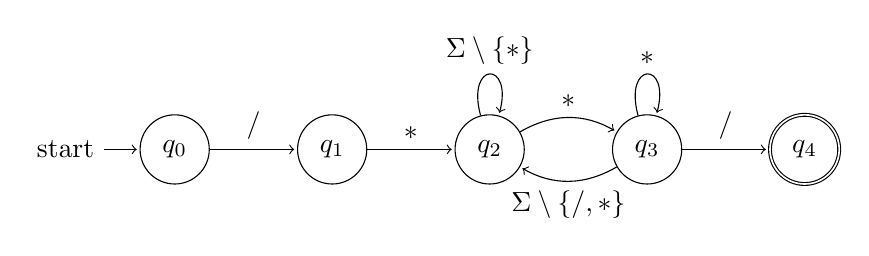
\begin{tikzpicture}[shorten >=1pt,node distance=2cm,on grid,auto]
		      \node[state,initial] (q_0) {$q_0$};
		      \node[state] (q_1) [right of=q_0] {$q_1$};
		      \node[state] (q_2) [right of=q_1] {$q_2$};
		      \node[state] (q_3) [right of=q_2] {$q_3$};
		      \node[state,accepting] (q_4) [right of=q_3] {$q_4$};

		      \path[->] (q_0) edge node {$/$} (q_1)
		                (q_1) edge node {$*$} (q_2)
		                (q_2) edge [bend left] node {$*$} (q_3)
		                edge [loop above] node {$\Sigma \setminus \{*\}$} ()
		                (q_3) edge [bend left] node {$\Sigma \setminus \{/,*\}$} (q_2)
		                edge [loop above] node {$*$} ()
		                edge node {$/$} (q_4);
		    \end{tikzpicture}
	    \end{center}
	    \caption{Example for a TikZ image; here using the \texttt{automata} library.}
	    \label{fig:tikz}
    \end{figure}
	Your first graphics in TikZ \emph{will} be time-eaters, but with some practice simple sketches are done in minutes.
	With a little bit of extra tuning, the same sources produce figures of unsurpassed quality.

  \item You can use document class \texttt{beamer} for creating presentation slides.
    It introduces some special syntax; best check the documentation and/or search the web.
\end{itemize}


\section{General research tools}

\begin{description}
	\item[\href{http://scholar.google.com}{Google Scholar} \& backwards search]
		~\\ % Cannot simply use \\ for newline as there would be an `empty' line ... therefore use ~\\
		Google Scholar can be used to find papers and books of all kinds and often has links to PDF versions that are freely available, e.\,g., on authors' websites.
		Moreover, Google Scholar can be used for finding other relevant articles in a field by backward-searching for papers that reference a given paper; see screenshot in Figure~\ref{fig:scholar}. % Use ~ for non-breaking space.
		Google Scholar has some basic support for exporting entries to BibTeX; the results often need some manual polishing, though.

		% Figures are placed by latex where they fit and should thus always be referenced by
		% the \label{}-\ref{} mechanism
		\begin{figure}
			\begin{center}
				\fbox{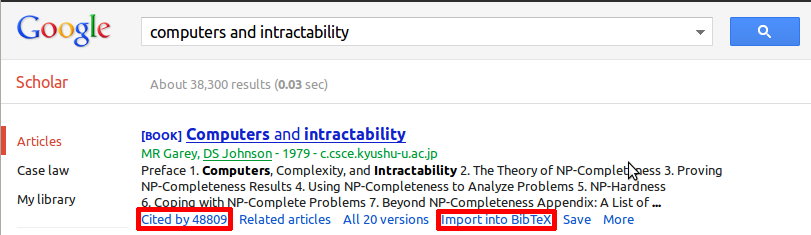
\includegraphics[width=.9\linewidth]{scholar}}%
				% fbox for "framed box"
			\end{center}
			\caption{%
				Some Google Scholar features we would like to highlight: back-references (find all papers that cite a given article) and BibTeX export (you may need to enable this in Google Scholar settings).
			}
			\label{fig:scholar} % NOTE: \label must appear after \caption
		\end{figure}

	\item[\href{http://dblp.uni-trier.de/}{dblp}] is a searchable index of computer science bibliography with BibTex entries for all articles.

	\item[\href{http://www.mendeley.com}{Mendeley}] is a (free) web service for storing references (including PDFs).

		The collected references can be exported to BibTeX.

	\item[aspell] or some other spell checker.

		As a general rule, typos that can be found by running a spell checker are unacceptable.

	\item[Git] or some other version control system (like Subversion)

		Very useful for keeping old versions around and highly recommended.
		It works best on text files, but can also handle binary files.
		A comprehensive introduction is available as free ebook \cite{gitbook}.

		Git repositories can easily be cloned, e.\,g., onto an external drive for backup.
		That way, you get incremental backups of your work basically for free.

		As Git (and all other versioning systems) typically operate in a \emph{line-based} way,
		it is very advisable to break your text into short lines ($\approx$\,100 character).
		For documents that are edited collaboratively, it has been good practice to start a new line for each sentence (or even sub-clause)%
		\footnote{%
		  Recall that a newline is treated by \LaTeX{} like an ordinary space.
		  Only empty lines indicate a new paragraph.
		}.

\end{description}


\section{Bibliography}
The section has been copied from the original template of the EPTCS style (\cite{bibliographystylewebpage}).

We request that you use \href{http://eptcs.web.cse.unsw.edu.au/eptcs.bst}{\texttt{$\backslash$bibliographystyle$\{$eptcs$\}$}}
\cite{bibliographystylewebpage}.
Compared to the original {\LaTeX} \texttt{$\backslash$biblio\-graphystyle$\{$plain$\}$}, it ignores the field \texttt{month}, and uses the extra bibtex fields \texttt{eid}, \texttt{doi}, \texttt{ee} and \texttt{url}.
The first is for electronic identifiers (typically the number $n$ indicating the $n^{th}$ paper in an issue) of papers in electronic journals that do not use page numbers.
The other three are to refer, with life links, to electronic incarnations of the paper.

Almost all publishers use digital object identifiers (DOIs) as a persistent way to locate electronic publications.
Prefixing the DOI of any paper with \url{http://dx.doi.org/} yields a URI that resolves to the current location (URL) of the response page\footnote{Nowadays, papers that are published electronically tend to have a \emph{response page} that lists the title, authors and abstract of the paper, and links to the actual manifestations of the paper (e.g.\ as \texttt{dvi}- or \texttt{pdf}-file).
Sometimes publishers charge money to access the paper itself, but the response page is always freely available.} of that paper.
When the location of the response page changes (for instance through a merge of publishers), the DOI of the paper remains the same and (through an update by the publisher) the corresponding URI will then resolve to the new location.
For that reason a reference ought to contain the DOI of a paper, with a life link to corresponding URI, rather than a direct reference or link to the current URL of publisher's response page.
This is the role of the bibtex field \texttt{doi}.
DOIs of papers can often be found through \url{http://www.crossref.org/guestquery}; the second method {\itshape Search on article title}, only using the {\bfseries surname} of the first-listed author, works best.

Often an official publication is only available against payment, but as a courtesy to readers that do not wish to pay, the authors also make the paper available free of charge at a repository such as \url{arXiv.org}.
In such a case it is recommended to also refer and link to the URL of the response page of the paper in such a repository.
This can be done using the bibtex fields \texttt{ee} or \texttt{url}, which are treated as synonyms.
These fields should not be used to duplicate information that is already provided through the DOI of the paper.
You can find archival-quality URL's for most recently published papers in DBLP --- they are in the bibtex-field \texttt{ee}.
In fact, it is often useful to check your references against DBLP records anyway, or just find them there in the first place.

%%%%%%%%%%%%%%%%%%%%%%%%%%%%%%%%%%%%%%%%%%%%%%%%%%%%%%%%%%%%%%%%%%%%%%%%%%%%%%%
\newpage
\nocite{*}
\bibliographystyle{eptcs}
\bibliography{references}

%%%%%%%%%%%%%%%%%%%%%%%%%%%%%%%%%%%%%%%%%%%%%%%%%%%%%%%%%%%%%%%%%%%%%%%%%%%%%%%
\end{document}
%%%%%%%%%%%%%%%%%%%%%%%%%%%%%%%%%%%%%%%%%%%%%%%%%%%%%%%%%%%%%%%%%%%%%%%%%%%%%%%
